%%%%%%%%%%%%%%%%%%%%%%%%%%%%%%%%%%%%%%%%%%%%%%%%%%%%%%%%%%%%%%%%%%%%%%%%%%%%%%%
%%%%%%%%%%%%%%%%%%%%%%%%%%%%%%%%%%%%%%%%%%%%%%%%%%%%%%%%%%%%%%%%%%%%%%%%%%%%%%% 
\chapter{Abelfunctions} \label{ch:abelfunctions}
%%%%%%%%%%%%%%%%%%%%%%%%%%%%%%%%%%%%%%%%%%%%%%%%%%%%%%%%%%%%%%%%%%%%%%%%%%%%%%%
%%%%%%%%%%%%%%%%%%%%%%%%%%%%%%%%%%%%%%%%%%%%%%%%%%%%%%%%%%%%%%%%%%%%%%%%%%%%%%%

The primary result of this thesis is the Sage software library Abelfunctions
\cite{abelfunctions}. The goal of Abelfunctions is to provide general and easy
to use framework for computing with Abelian functions, Riemann surfaces, and
algebraic curves.

Abelfunctions was inspired by the Maple software package Algcurves developed by
Deconinck, van Hoeij, and Patterson \cite{DeconinckPatterson11}. The need for
Abelfunctions grew out of the difficulty in keeping Algcurves up to date within
Maple's proprietary software. Because of the need to resolve issues as they are
encountered as well as allowing the ability to improve upon the software when
new algorithms are developed, Abelfunctions was created using a completely
open-source model within completely open-source software.

Abelfunctions differs from Algcurves in two main ways. First, the opportunity
write a new a software package for computing with Riemann surfaces invites the
opportunity to investigate better software design. The philosophy of design is
first influenced by the choice of the Python/Sage language which offers features
not availble in Maple. Furthermore, the use of object-oriented design offers the
ability to more easily improve upon Abelfunctions in the future. Following these
well-studied object-oriented design patterns \cite{gamma1995design} is in line
with the reproducibility movement spreading in the computational sciences
\cite{stodden2012reproducible} which encourages the release of well-designed and
well-documented code used in any scientific endeavor which makes use of
computational results.

Second, the opportunity to implement the functionality of Algcurves in a
different environment provided the opportunity to improve upon existing
algorithms. The path from plane algebraic curve to period matrix, Abel map, and
Riemann constant vector draws from a diverse set of algorithms used to realize
the intermediate steps leading to these goals.

In this chapter we will take a closer look at the software design and algorithm
implementation details of the package. In Section \ref{sec:reproducibility} we
begin with a discussion on reproducible research and its motivating role in the
creation of Abelfunctions. In Section \ref{sec:object-oriented-design} we give a
short introduction to object-oriented design and highlight the key patterns and
techniques used to improve reproducibility. Section
\ref{sec:abelfunctions-a-tour-of-abelfunctions} is the ``developer's guide''
where we explore the design and organization of Abelfunctions. Finally, in
Section \ref{sec:abelfunctions-improvements-on-algorithms} we highlight the
algorithmic improvements made on previous work in the field.

The Abelfunctions source code can be found on GitHub at
\url{http://github.com/abelfunctions}.


%%%%%%%%%%%%%%%%%%%%%%%%%%%%%%%%%%%%%%%%%%%%%%%%%%%%%%%%%%%%%%%%%%%%%%%%%%%%%%%
\section{Reproducibility and Scientific Software Design}\label{sec:reproducibility}
%%%%%%%%%%%%%%%%%%%%%%%%%%%%%%%%%%%%%%%%%%%%%%%%%%%%%%%%%%%%%%%%%%%%%%%%%%%%%%%

Reproducibility is standard practice in the physical sciences. When sharing
research with the scientific community one should provide sufficient detail of
the experimental setup, performance metrics, and observations for a second party
to repeat the experiment. Whatever the state of reproducibility is in physical
science some have observed that field of computational science is lagging
behind. From the generation of figures to the demonstration of newly developed
algorithms many papers display these results without providing the means of
generating these data: the source code.

During the development of WaveLab, Buckheit and Donoho created the following
slogan,
\begin{quotation}
  An article about computational science in a scientifc publication is not the
  scholarship itself, it is merely advertising of the scholarship. The actual
  scholarship is the complete software development environment and the complete
  set of instructions which generated the figures \cite{buckheit1995wavelab}.
\end{quotation}
The [XXX][FINISH]

To read more about the reproducibility movement in computational science see
\cite{peng2011reproducible}, \cite{stodden2012reproducible}, and
\cite{stodden2013best}.


%%%%%%%%%%%%%%%%%%%%%%%%%%%%%%%%%%%%%%%%%%%%%%%%%%%%%%%%%%%%%%%%%%%%%%%%%%%%%%%
\section{A Brief Look at Object-Oriented Design}\label{sec:object-oriented-design}
%%%%%%%%%%%%%%%%%%%%%%%%%%%%%%%%%%%%%%%%%%%%%%%%%%%%%%%%%%%%%%%%%%%%%%%%%%%%%%%

Many applied mathematician write code but do not necessarily write
object-oriented code. Sometimes this is a restriction imposed by the language of
choice. For example, Lisp and Scala, programming languages popular in the
artificial intelligence communities, are not object-oriented languages. Other
times, it is due to an unawareness of its existence or utility. This section
provides an introduction to object-oriented programming and design for
computational scientists and why it is useful in scientific code. In particular,
we will see examples where this software design tool is used to produce reusable
scientific software and avoid rotting design. It is suggested that readers of
this section have some programming experience, preferrably in Python or Sage.

Robert Martin succinctly addresses what goes wrong with software once it
achieves non-trivial levels of complexity in a list of four symptoms of rotting
design \cite{martin2000design}. The common element across these symptoms is that
rotting design adds developer time and reduces manager and customer trust.
\begin{itemize}
\item {\bf Rigidity} - the tendency for software to be difficult to change. When
  a simple fix should take several days but instead takes weeks, managers and
  advisors are reluctant to let developers address non-critical issues.
\item {\bf Fragility} - the tendency for software to break, potentially in many
  places, every time it is changed. Fragile software creates connections between
  parts of code that are supposed to be logically distinct.
\item {\bf Immobility} - the inability to reuse software from parts of other
  projects or the same project. The more extraneous components a software
  component has the less potential it has to be generalized.  When 
  immobility is high the amount of work required to separate out potentially
  resuable parts of code is greater than the work it takes to rewrite the code
  entirely.
\item {\bf Viscosity} - the situation where, when making a code change, the
  approach that preserves the software design is more expensive than the
  approach that does not. Viscous software encourages ``hacks'' as solutions to
  problems rather than coherent modifications.
\end{itemize}

Object-oriented languages, such as Python and Sage, provide the ability to form
abstractions of data and functionality for the purposes of reusability and
modularity. When used correctly one avoids rotting design traps. The main
concepts of object-oriented programming are objects, classes, inheritance, and
polymorphism.

Design patterns are methodologies for writing object-oriented code so as to
avoid rotting design. A complete overview of design patterns is beyond the scope
of this text. The curious reader is encouraged to read \cite{gamma1995design}
for an encyclopedia of design patterns for many common design situations and
\cite{martin2000design} for a list of general strategies to avoid introducing
rot into your system.



\subsection{Objects and Classes}

Objects are the basic entities in an object oriented system. They represent the
combination of data and operations acting on these data. When a program is
executed objects interact with each other by sending messages. Objects have two
components: state and behavior. The state of an object is any data that it may
encapsulate and the behavior consists of functions, often called methods, that
use the state to communicate information to the user and to other objects.

Objects are instances of classes which define the state format and available
behaviors. For example, a \verb=Person= class may consist of two data fields,
\verb=name:string= and \verb=age:int=, and a method \verb=speak()= which returns
the string \verb='My name is <name> and I am <age> years old.'=. A class diagram
[XXX] can be used to graphically represent this class.

% TODO: insert class diagram

Two objects, \verb=Alice= and \verb=Bob=, are instances of the \verb=Person=
class with the \verb=name= field defined as \verb='Alice'= and \verb='Bob'=,
repectively, and given definitions for \verb=age= as well. Note that the
\verb=speak()= method does not differ between the two objects. Instead, it uses
the data defined by the objects to return the appropriate string message.

In the remainder of this section we will use a more interesting running example
of building an numerical integrator package in order to motivate the use of
object-oriented design principles. The implementation details will be
omitted we instead focuson the software structure.

%------------------------------------------------------------------------------
\subsection{Inheritance}
%------------------------------------------------------------------------------

Suppose we wanted to write a piece of scientific software implementing several
numerical integration techniques. The use provides a function {\tt func} and the
software package will numerically integrate the function using a chosen
algorithm. If an algorithm is not provided then a default algorithm is chosen
for the user.

The novice programmer might write a function along the following lines,
\begin{lstlisting}
def integrate(f, method_name):
    if method_name = 'newton_cotes':
        # integrate func using the Newton Cotes method
    else if method_name = 'gaussian_quadrature':
        # integrate func using the Gaussaian Quadrature method
    else if method_name = 'clenshaw_curtis':
        # integrate func using the Clenshaw Curtis Quadrature method
    else
        # integrate using default technique (Newton Cotes)

    return integral
\end{lstlisting}
This approach would work, and a certain class of engineer may deem this
acceptable, but may be difficult to work on. One practical issue is that the
{\tt integrate} function may become too long and thus increasingly difficult to
debug. The developer would have to keep track of which lines of code
corresponded to which numerical integration technique.

One obvious improvement is to break out each of the integration methods into a
separate function.
\begin{lstlisting}
def integrate(func, method_name):
    if method_name = 'newton_cotes':
        integral = integrate_newton_cotes(func)
    else if method_name = 'gaussian_quadrature':
        integral = integrate_gaussian_quadrature(func)
    else if method_name = 'clenshaw_curtis':
        integral = integrate_clenshaw_curtis(func)
    else
        integral = integrate_newton_cotes(func)

    return integral

def integrate_newton_cotes(func):
    # integrate func using the Newton Cotes method
    return integral
    
def integrate_gaussian_quadrature(func):
    # integrate func using the Gaussian Quadrature method
    return integral
    
def integrate_clenshaw_curtis(func):
    # integrate func using the Clenshaw Curtis method
    return integral
\end{lstlisting}
This is an improvement from an organizational perspective. However, imagine the
following situation: a contributor wants to implement a new numerical
integrator. They write a function \verb=integate_my_technique=. But to integrate
it into the primary {\tt integrate()} function they would need to modify the
source code of {\tt integrate()}.

In this simple example this may not be an issue. However, moving beyond this toy
situation reveals potential issues. If the definition of {\tt integate()}
existed in a different source file than the contributor would need to find it
and add an \verb=else..if= conditional to the growing list. An ad hoc solution
would be for the developer to provide documentation of this situation. %TODO




One class of numerical integrators are of the form
\[
  \int_{-1}^1 f(x) dx \approx \sum_{i=0}^n w_i f(x_i)
\]
where the weights $w_i$ and evaluation locations $x_i$ are chosen based on the
technique used. For example,
\begin{itemize}
\item {\bf Degree $2$ Newton-Cotes (Trapezoid Rule)} - $w_i = 1$ if $i=0$ or
  $i=n$ and $w_i = 2$ otherwise, and $x_i = -1 + 2i/n$.
  \item {\bf Gaussian Quadrature} - $w_i = 1/\sqrt{1-x_i^2}$
\end{itemize}


\begin{lstlisting}
class NumericalIntegrator(object):
    def __init__(self, n):
        self.n = n

    def weights(self):
        raise NotImplementedError()

    def integrate(self, func):
        w, x = self.weights_and_locations()
        return sum(w[i]*func(x[i]) for i in range(n))
\end{lstlisting}


\begin{lstlisting}
class NewtonCotesQuadrature(NumericalIntegrator):
    def weights(self):
        # return the newton coates quadrature weights, w
        return w

class GaussianQuadrature(NumericalIntegrator):
    def weights(self):
        # return the gaussian quadrature weights, w
        return w

class ClenshawCurtisQuadrature(NumericalIntegrator):
    def weights(self):
        # return the clenshaw curtis quadrature weights, w
        return w
         
\end{lstlisting}

Such a system is easily extendible: if a user or developer devises a new
numerical integration technique they need only to create a new subclass of {\tt
  NumericalQuadrature} and pass instances of that subclass to the appropriate
functions.

This design avoids the four rotting design symptoms:
\begin{itemize}
\item {\bf Rigidity} - adding a new integrator does not require changing code in
  multiple locations.
\item {\bf Fragility} - although this example is relatively simple, as long as
  the new integrator adheres to the data contract of {\tt
    NumericalQuadrature.integrate()} it will not break the software.
  Furthermore, the design makes it easy to test the new integrator directly.
\item {\bf Immobility} - the integration logic is separated from its uses in
  other parts of the code. 
\item {\bf Viscosity} - separating the integration logic from the rest of the
  code allows the developer to isolate and better control the interface to these
  components. {\tt NumericalQuadrature} makes it clear how functions are
  integrated.
\end{itemize}

% TODO - mention design contract below...explain?
% TODO - really messy train of thought. clean up


      

\subsection{Composition}

\subsection{Strategy Design Pattern}

\subsection{Dependency Inversion}


%%%%%%%%%%%%%%%%%%%%%%%%%%%%%%%%%%%%%%%%%%%%%%%%%%%%%%%%%%%%%%%%%%%%%%%%%%%%%%%
\section{A Tour of Abelfunctions}\label{sec:abelfunctions-a-tour-of-abelfunctions}
%%%%%%%%%%%%%%%%%%%%%%%%%%%%%%%%%%%%%%%%%%%%%%%%%%%%%%%%%%%%%%%%%%%%%%%%%%%%%%%

Abelfunctions several top-level functions and objects. The user takes advantage
of the Abelfunctions functionality primarily through these objects.
\begin{itemize}
  \item {\tt RiemannSurface} - principle object, defines a Riemann surface given
    a bivariate Sage polynomial.
  \item {\tt AbelMap} - defines the Abel map function from one place on a
    Riemann surface to another. Can accept divisors as well.
  \item {\tt RiemannConstantVector} - defined the Riemann constant vector
    function as a function of an arbitrary place on a Riemann surface.
  \item {\tt RiemannTheta} - the Riemann theta function as a function from
    $\CC^g \times \hg$ to $\CC$.
\end{itemize}

\noindent We begin by importing this functionality and constructing a Riemann
surface corresponding to the plane algebraic curve,

\[
  C : x^2y^3 - x^4 + 1 = 0, \quad x,y \in \CC^*.
\]

\begin{lstlisting}[language=Sage]
sage: from abelfunctions import *  # import the main Abelfunctions functionality
sage: R.<x,y> = QQ[]  # construct a Sage polynomial ring and the above curve
sage: f = y**3 - 2*x**3*y + x**7
sage: X = RiemannSurface(f); X  # construct the corresponding Riemann surface
Riemann surface defined by f = x^7 - 2*x^3*y + y^3
\end{lstlisting}

\noindent The genus of the curve is determined using the singularity structure.
In this case, the Riemann surface is of genus four.

\begin{lstlisting}[language=Sage]
sage: g = X.genus(); g
4
\end{lstlisting}

\noindent We can verify this with the singularity data.

\begin{lstlisting}[language=Sage]
sage: from abelfunctions.singularities import singularities
sage: for point, (m, delta, r) in singularities(f):
 ...:     print point, '\tdelta invariant =', delta
(0, 1, 0)    delta invariant = 2
sage: d = f.total_degree()
sage: g = (d-1)*(d-2)/2 - 2  # (-2) from the delta inv. above
sage: g
4
\end{lstlisting}

%------------------------------------------------------------------------------
\subsection{Places and Divisors}
% ------------------------------------------------------------------------------


%%%%%%%%%%%%%%%%%%%%%%%%%%%%%%%%%%%%%%%%%%%%%%%%%%%%%%%%%%%%%%%%%%%%%%%%%%%%%%%
\section{Algorithms}\label{sec:abelfunctions-algorithms}
%%%%%%%%%%%%%%%%%%%%%%%%%%%%%%%%%%%%%%%%%%%%%%%%%%%%%%%%%%%%%%%%%%%%%%%%%%%%%%%

This section is the algorithmic equivalent to
\autoref{sec:background-algebraic-curves-and-riemann-surfaces}. Here we present
the algorithms used to computationally realize Riemann surfaces, the Abel map,
and the Riemann theta function.

%%%%%%%%%%%%%%%%%%%%%%%%%%%%%%%%%%%%%%%%%%%%%%%%%%%%%%%%%%%%%%%%%%%%%%%%%%%%%%%
\subsection{Puiseux Series}\label{subsec:abelfunctions-puiseux-series}
%%%%%%%%%%%%%%%%%%%%%%%%%%%%%%%%%%%%%%%%%%%%%%%%%%%%%%%%%%%%%%%%%%%%%%%%%%%%%%%

The algorithm used in Abelfunctions for computing truncations of Puiseux series
expansions is based on that of Duval \cite{Duval89}. The main ingredient of the
algorithm are Newton polygons of algebraic curves. We give a brief outline of
the process here.
\begin{itemize}
\item The goal of the algorithm is to compute a list of tuples $\pi = (\tau_1,
  \tau_2, \ldots, \tau_R)$ where $\tau_i = (q_i,\mu_i,m_i,\beta_i,\eta_i)$.
  These tuples define the relations
  \begin{align*}
    X_{i-1} &= \mu_i X_i^{q_i}, \\
    Y_{i-1} &= (\beta_i + \eta_iY_i)X_i^{m_i},
  \end{align*}
  where $i = 1, \ldots, R$. To obtain the desired Puiseux series we set $x =
  X_0$, $y = Y_0$, and $t = X_R$ and eliminate the intermediate variables
  $X_1,\ldots,X_{R-1}$ and $Y_1,\ldots,Y_{R-1}$.
\item The first set of $\tau_i$ computed are those representing the {\it
    singular part} of $P$, that is, the part of the series if the Puiseux series
  has a ramification index $|e_j|>1$. This is done using the Newton polygon
  method. The output of this stage of the algorithm provides enough information
  to distinguish the Puiseux series expansions at $x=\alpha$.
\item Finally the algorithm computes the {\it regular} terms of the Puiseux
  series using a standard Taylor series techniques.
\end{itemize}


%%%%%%%%%%%%%%%%%%%%%%%%%%%%%%%%%%%%%%%%%%%%%%%%%%%%%%%%%%%%%%%%%%%%%%%%%%%%%%%
\subsection{Singularities}\label{subsec:abelfunctions-singularities}
%%%%%%%%%%%%%%%%%%%%%%%%%%%%%%%%%%%%%%%%%%%%%%%%%%%%%%%%%%%%%%%%%%%%%%%%%%%%%%%


First we determine the finite singularities of $C : f(x,y) = 0$. Let $R(x)$ be
the resultant of $f(x,y)$ and $\partial_y f(x,y)$ \cite{Griffiths89}. We compute
the roots
\begin{align*}
    S &= \{ x \in \CC \; | \; R(x) = 0, \partial_x R(x) = 0 \} \\
      &= \{ x_1, \ldots, x_s \}.
\end{align*}
For each $x_j \in S$ we compute the $y$-roots $\{y_{j1},\ldots,y_{jd}\}$
where $d = \text{deg}_y f$. The places $(x_j,y_{jk})$, $j=1,\ldots,s$,
$k=1,\ldots,d$ satisfy
\[
    f(x_j,y_{jk}) = 0, \quad \partial_y f(x_j,y_{jk}) = 0,
\]
by the definition of the resolvent. Therefore, the singular places
$(x_k,y_{jk})$ are those that satisfy
\[
    \partial_x f(x_j,y_{jk}) = 0.
\]
By definition, these remaining places are the finite singular points of the
curve $C$. For the infinite case we use the projection of the curve on the line
at infinity. (See Section \ref{sec: projective-plane-curves}.)

%% To compute the branching number of a singular point $(\alpha,\beta)$ we
%% simply calculate the sum of the ramification indices at all Puiseux series
%% $P_j$ such that $P_j(0) = (\alpha,\beta)$.

%% We can also use Puiseux series to compute the multiplicity of a singular point.

The methods used to compute the branching number, multiplicity, and delta
invariant of a singularity rely on examining the leading order behavior of the
Puiseux series expansions such that $P_j(0) = (\alpha, \beta)$. For the details
of these methods see \cite{DeconinckPatterson11}. In brief the branching number
$R$ of singularity is computed using the above formula
\[
  R \quad = \sum_{\substack{j \\ P_j(0)=(\alpha,\beta)}} |e_j|.
\]
The multiplicity is the sum of the minimum of $e_j$ and $n_{jN}$ over all
Puiseux series $P_j$ such that $P_j(0) = (\alpha,\beta)$ where $\beta_{jN} t
^{n_{jN}}$ is the first non-zero, non-constant term appearing the in $y_j$. The
delta invariant is equal to
\[
    \delta = \frac{1}{2}\sum_{j=1}^m r_j \text{Int}_{P_j} - r_j + 1,
\]
where
\[
  \text{Int}_{P_j} = \sum_{k=1^d, k \neq j} \text{val}_x \big( y_j(x) -
  \tilde{y}_k(x) \big),
\]
with $\text{val}_x( g(x))$ equal to the lowest exponent of $x$ appearing in
$g(x)$, and $y_j(x)$ is the $y$-part of $P_j$ when solving for $t = t(x)$. The
sum appearing in $\text{Int}_{P_j}$ is taken over {\it all} Puiseux series
expansions $P_k$ at $x = \alpha$, not just the ones with $P_k(0) = (\alpha,
\beta)$.


%%%%%%%%%%%%%%%%%%%%%%%%%%%%%%%%%%%%%%%%%%%%%%%%%%%%%%%%%%%%%%%%%%%%%%%%%%%%%%%
\subsection{Analytic
  Continuation}\label{subsec:abelfunctions-analytic-continuation}
%%%%%%%%%%%%%%%%%%%%%%%%%%%%%%%%%%%%%%%%%%%%%%%%%%%%%%%%%%%%%%%%%%%%%%%%%%%%%%%


To compute a path $\gamma$ on a Riemann surface $C$ we provide a continuous
$x$-path $x_\gamma(t)$ and an initial $y$-value $y_0$ as input and we wish to
receive the resulting $y$-path $y_\gamma(t)$ as output. Analytic continuation of
$y_0$ along $\gamma$ is a fundamental operation in Abelfunctions since
evaluation of and integration along paths is done frequently. Therefore, it is
important to make the construction and evaluation along paths as fast and
efficient as possible.

We use numerical methods to estimate values along $y_\gamma(t)$. In general, the
problem is phrased as given $\gamma(t_i) = (x_i,y_i)$ as well as some later
$t_{i+1} = t_i + \Delta t$ and $x_{i+1} = x_\gamma(t_{i+1})$ determine the value
$y_{i+1} = y_\gamma(t_{i+1})$.

A first and natural approach to solving this problem is to use a root finder.
Given $x_{i+1}$ we numerically or symbolically solve the equation
\[
  f(x_{i+1},y) = 0.
\]
This produces $n$ $y$-roots $y_{i+1,1}, \ldots, y_{i+1,d}$ over $x_{i+1}$.
However, even if one finds an effective and fast method for doing this with
arbitrary degree polynomials $f$, the main problem with this approach is
determining which $y_{i+1,k}$ is equal to the desired root $y_{i+1}$. One could
argue that the desired root is the one minimizing $|y_{i+1,k} - y_i|$ (the root
closest to the previous $y$-root) but it is conceivable that this closest can
change as a function of $\Delta t$, especially if $\Delta t$ is too large.

Another approach could be to use Newton iteration: given $x_{i+1}$ and an {\it
  initial guess} $y_i$ at $x_i$ use Newton iteration on the function $g(y) =
f(x_{i+1}, y)$ to determine $y_{i+1}$. However, this approach suffers from the
same problem, namely, the root $y_{i+1,k}$ produced by Newton iteration may
change as a function of $\Delta t$. Too large of a $\Delta t$ may result in {\it
  branch jumping}, where we converge to the incorrect $y$-root. Too small of a
$\Delta t$ gives an inefficient numerical algorithm. Further, the definition of
``small enough'' may change as a function of the curve $C$ and the $x$-points
$x_{i}$ and $x_{i+1}$.

To solve the problem of selecting an appropriate $\Delta t$ we use Smale's
$\alpha$-theory \cite{Smale85}. The purpose of Smale's $\alpha$-theory is to
answer the following questions about $g(y) = f(x_{i+1},y)$ for some finite set
of points $Y \subset \CC$:
\begin{enumerate}
\item From which points in $Y$ will Newton's method converge quadratically to
  some solution to $g$?
\item From which points in $Y$ will Newton's method converge quadratically to
  distinct solutions to $g$?
\item If $g$ is real ($\bar{g} = g$), from which points of $Y$ will Newton's
  method converge quadratically to real solutions to $g$?
\end{enumerate}
See \cite{HauensteinSottile10} for an excellent summary of Smale's
$\alpha$-theory. Using the notation of Hauenstein and Sottile, we outline the
analytic continuation algorithm here.
\begin{enumerate}
\item Assume we know the {\it $y$-fibre} $y_i = \{y_{i,1},\ldots,y_{i,d}\}$ of
  $g_i(y) := f(x_i,y)=0$. Fix some initial $\Delta t$ and let $x_{i+1} =
  x_\gamma(t_i + \Delta t)$. We wish to compute the $y$-fibre $y_{i+1}$ of
  $g_{i+1}(y) := f(x_{i+1},y)$ such that each element $y_{i+1,j}$ is the
  analytic continuation of $y_{i,j}$ to $x_{i+1}$.
\item We first determine if the $y$-fibre $y_i$ is an {\it approximate solution}
  to $g_{i+1}(y) = 0$. Does each element of $y_i$ lie in the quadratic
  convergence region of Newton's method on $g_{i+1}$?

  If not, return to Step (1) with $\Delta t \mapsto \Delta t / 2$.
\item Next, determine if the approximate solutions $y_{i,j}$ will converge to
  distinct associated solutions $y_{i+1,j}$: will the approximate solutions jump
  branches or stay on their respective branches?

  If not, return to Step (1) with $\Delta t \mapsto \Delta t / 2$.
\item The $y$-fibre satisfies the necessary conditions for Newton iteration to
  converge to the appropriate analytic continuations $y_{i+1,j}$ at $x_{i+1}$.
  Newton iterate and output this solution $y$-fibre.
\end{enumerate}

Note that this algorithm requires analytically continuing all of the $y$-roots
along an $x$-path in the complex plane since we cannot determine an appropriate
step size for continuing a given root without knowing the locations of the other
roots. Although this impacts the performance of the algorithm since we have to
perform $d$ sets of Newton iterations at each step, Smale's $\alpha$-theory
provides a rigorous method for determining an appropriate step size.


%%%%%%%%%%%%%%%%%%%%%%%%%%%%%%%%%%%%%%%%%%%%%%%%%%%%%%%%%%%%%%%%%%%%%%%%%%%%%%%
\subsection{Monodromy}\label{subsec:abelfunctions-monodromy}
%%%%%%%%%%%%%%%%%%%%%%%%%%%%%%%%%%%%%%%%%%%%%%%%%%%%%%%%%%%%%%%%%%%%%%%%%%%%%%%


The algorithm implemented in Abelfunctions for computing the monodromy
group of a curve is based on the one described in \cite{FKS12}. Due to the
technical nature of the algorithm only a summary is provided here.

\begin{itemize}
\item We require that the monodromy paths constructed stay sufficiently far from
  the branch points due to the numerical accuracy of Newton's method when used
  in the analytic continuation process. For each branch point, $b_i$ we let
  \[
    \rho_i = \text{min}_{\substack{j=1,\ldots,n \\ j\neq i}} |b_i - b_j|.
  \]
  The minimal distance that any path $x_\gamma$ be from the branch point $b_i$
  is
  \[
    R_i = \frac{\rho_i \kappa}{2}
  \]
  where $\kappa \in (0,1]$ is a chosen relaxation factor. The implementation of
  this algorithm in Abelfunctions uses $\kappa = 3/5$.
\item Let $b = b_i$ be the branch point where $\re b_i < \re b_j$ for all $j
  \neq i$. The point $b$ is referred to as the {\it base branch point}. Choose
  the base point $\alpha_0$ to be the point $\alpha_0 = b - R_b$, the point on
  the minimal distance circle encircling $b$.
\item Order the remaining branch points $\{b_j\}_{j \neq i}$ by increasing
  argument with $b$. This ordering determines the ordering of the monodromy
  paths $x_{\gamma_j}$.
\item Construct a complete graph $G$ with the branch points $b_1,\ldots,b_n$ as
  nodes and compute the minimal spanning tree $T$ of this graph with $b$ as the
  parent node.
\item Using line segments and semi-circles, construct the path $x_{\gamma_j}$
  encircling $b_j$ once in the positive direction by starting at the base point,
  following the minimal spanning tree to $b_j$ and using semicircles to traverse
  over or under the branch points along the way depending on the ordering. That
  is, the path $x_{\gamma_j}$ should be constructed in such a way so that the
  branch points $b_1,\ldots,b_{j-1}$ lie below the path.
\item Fix an ordering of the base fibre $(y_0,\ldots,y_{d-1})$ above $\alpha_0$
  and analytically continue around each $x_{\gamma_j}$ to determine the
  permutations $\pi_j$.
\end{itemize}


%%%%%%%%%%%%%%%%%%%%%%%%%%%%%%%%%%%%%%%%%%%%%%%%%%%%%%%%%%%%%%%%%%%%%%%%%%%%%%%
\subsection{Homology}\label{subsec:abelfunctions-homology}
%%%%%%%%%%%%%%%%%%%%%%%%%%%%%%%%%%%%%%%%%%%%%%%%%%%%%%%%%%%%%%%%%%%%%%%%%%%%%%%


Tretkoff and Tretkoff \cite{TretkoffTretkoff84} provide an algorithm for
determining a canonical cycle basis for $H_1(X,\ZZ)$ given the monodromy group
of a curve. We omit the details of the algorithm here. At its core, it computes
a graph which encodes how to travel from the {\it base place} of $X$, chosen to
be
\[
  P_0 = (\alpha_0, \beta_0)
\]
where $\alpha_0$ is the base point of the monodromy group of the curve and
$\beta_0 = y_0$ is a fixed root lying above $x = \alpha_0$, to the other places
$(\alpha_0, y_i)$ lying above $x = \alpha_0$ via traversal around one or more
branch points. (These places are sometimes called the {\it sheets} of the
surface $X$ with the $i$th sheet referring to the place $(\alpha_0,y_i)$). A
minimal spanning tree of this graph is computed where each removed edge
corresponds to a cycle in $H_1(X,\ZZ)$. The is because the addition of an edge
to the minimal spanning tree forms a cycle in the graph. This graph cycle in
turn represents a possibly a non-zero cycle on $X$. A separate part of the
algorithm is then used to compute a canonical basis of cycles by taking
appropriate linear combinations of these intermediate cycles.


%%%%%%%%%%%%%%%%%%%%%%%%%%%%%%%%%%%%%%%%%%%%%%%%%%%%%%%%%%%%%%%%%%%%%%%%%%%%%%%
\subsection{Holomorphic and Meromorphic
  Differentials}\label{subsec:background-holomorphic-and-meromorphic-differentials}
%%%%%%%%%%%%%%%%%%%%%%%%%%%%%%%%%%%%%%%%%%%%%%%%%%%%%%%%%%%%%%%%%%%%%%%%%%%%%%%

One condition on the $p_k$'s is immediately apparent: to preserve holomorphicity
$p_k$ must have a zero, with sufficient multiplicity, at the places $P =
(\alpha,\beta)$ where $\partial_y f(x,y)$ vanishes. More precisely, Noether
showed that if a singular place $P$ has multiplicity $m_P$ then $P_k$ must have
a zero of order at least $m_P - 1$ at $P$ \cite{Noether83}.

The technique we use to determine the adjoint polynomials $p_k$ uses a theorem
of M\~{n}uk relying on computing an integral basis for the algebraic function
field of the curve \cite{Mnuk97}. Let $A(C)$ be the {\it coordinate ring}
\[
  A(C) = \CC[x,y] / (f)
\]
of the curve $C : f(x,y) = 0$. The coordinate ring can be though of as the ring
of all functions $g \in \CC[x,y]$ vanishing on the curve $f$. Note that $A(C)$
is a subset of the {\it algebraic function field} $\CC(x,y)$.

Given a ring $R$ and a field $S$ such that $R \subset S$, the {\it integral
  closure $\bar{R}$ of $R$ in $S$} is the ring of all elements $s \in S$ such
that
\[
  s^n + r_{n-1}s^{n-1} + \cdots + r_1 s + r_0 = 0,
\]
for some choice of $n >0$ and $r_0,\ldots,r_{n-1} \in R$. That is $\bar{R}$
consists of all elements in $S$ satisfying some monic polynomial equation with
coefficients in $R$. Here, we consider the integral closure $\overline{A(C)}$ of
$A(C)$ in $\CC(x,y)$.

Again, we wish to find the set of all adjoint polynomials of $C$. By
\cite{Mnuk97}, these are the set of all $p \in \CC[x,y]$ such that
\[
  \overline{A(C)} p(x,y) \subset\CC[x,y].
\]
That is, all of the polynomials $p$ such that every element of
$\overline{A(C)}$, when multiplied by $p$ and reduced modulo $f(x,y)$, results
in a polynomial. Now, $\overline{A(C)}$ is a finite extension of $A(C)$.
Therefore,
\[
  \overline{A(C)} = \beta_1 A(C) + \cdots + \beta_m A(C), \quad \beta_k \in
  \CC(x,y).
\]
for an appropriate choice of $\beta_k$'s in $\CC(x,y)$. The set
$\{\beta_1,\ldots,\beta_m\}$ is called the {\it integral basis} of the integral
closure of the coordinate ring. Thus, finding the set of adjoint polynomials is
equivalent to finding polynomials $p \in \CC[x,y]$ such that
\[
  \beta_k(x,y) p(x,y) \in \CC[x,y], \quad \forall j=1,\ldots,m.
\]

To compute the adjoint polynomials we write
\[
  p(x,y) = \sum_{i+j \leq d-3} c_{ij}x^iy^j
\]
where $d = \text{deg}_y f$. We compute an integral basis
$\{\beta_1,\ldots,\beta_m\}$ for $\overline{A(C)}$ using the algorithm of van
Hoeij \cite{vanHoeij94}. The requirement that
\[
  \beta_k(x,y) \sum_{i+j \leq d-3} c_{ij}x^iy^j \in \CC[x,y]
\]
imposes a number of conditions on the coefficients $c_{ij}$ appearing in the
expression for $p(x,y)$. The set of all possible $c_{ij}$'s satisfying these
conditions for every $\beta_k, k=1,\ldots,m$ gives us the adjoint polynomials we
need.


%%%%%%%%%%%%%%%%%%%%%%%%%%%%%%%%%%%%%%%%%%%%%%%%%%%%%%%%%%%%%%%%%%%%%%%%%%%%%%%%
\subsection{Computing on the Period
  Lattice}\label{subsec:abelfunctions-period-lattice}
%%%%%%%%%%%%%%%%%%%%%%%%%%%%%%%%%%%%%%%%%%%%%%%%%%%%%%%%%%%%%%%%%%%%%%%%%%%%%%%

To compute $A_{ij}, B_{ij}$ we first a method for numerically integrating
holomorphic differentials over any given path $\gamma \subset C$. We only
consider finite paths on the curve: paths with finite $x$- and $y$-components.
Any such path can be parameterized by some parameter $t \in [0,1]$. Let
\[
  \gamma : [0,1] \to C, \quad \gamma(t) = \Big( x_\gamma(t),
  y_\gamma\big(x_\gamma(t)\big) \Big).
\]
(Recall that we treat $y$ as the dependent variable in $f(x,y)=0$.) Given this
parameterization, we compute the integral of a holomorphic differential
$\omega$. Letting $x$ and $y$ represent the local coordinates in $\CC^2$ we have
\begin{align}
  \int_\gamma \omega
  &=
    \int_\gamma \omega\big(x,y(x)\big)dx \notag \\
  &=
    \int_0^1 \omega \Big(
    x_\gamma(t), y_\gamma\big(x_\gamma(t)\big) \Big)
    \frac{dx_\gamma}{dt}(t) dt. \label{eqn: path-integral}
\end{align}

In Abelfunctions we construct paths $\gamma \subset C$ where $x_\gamma$ either
parameterizes a line from some $z_0\in\CC$ to $z_1\in\CC$
\[
  x_\gamma(t) = z_0(1-t) + z_1t,
\]
or arcs on a circle of radius $R$ with center $w\in\CC$
\[
  x_\gamma(t) = w + Re^{i(\theta + t \Delta \theta)}
\]
where $\theta$ is the starting angle and $\theta + \Delta \theta$ is the ending
angle on the circle. We use the analytic continuation methods described in
Section \ref{sec: analytic-continuation} to compute $y_\gamma(x_\gamma(t))$.
Finally, to compute the integral in Equation \eqref{eqn: path-integral} we use a
numerical integrator of choice. Abelfunctions allows one to use any
numerical integrator provided by the {\tt scipy} Python package that can  % TODO
                                % NOT SCIPY
integrate complex-valued functions. The Romberg method \cite{wiki:Romberg} is
chosen by default.


%%%%%%%%%%%%%%%%%%%%%%%%%%%%%%%%%%%%%%%%%%%%%%%%%%%%%%%%%%%%%%%%%%%%%%%%%%%%%%%%
\subsection{The Abel Map}\label{subsec:abelfunctions-abel-map}
%%%%%%%%%%%%%%%%%%%%%%%%%%%%%%%%%%%%%%%%%%%%%%%%%%%%%%%%%%%%%%%%%%%%%%%%%%%%%%%


%%%%%%%%%%%%%%%%%%%%%%%%%%%%%%%%%%%%%%%%%%%%%%%%%%%%%%%%%%%%%%%%%%%%%%%%%%%%%%%%
\subsection{Riemann Constant
  Vector}\label{subsec:abelfunctions-riemann-constant-vector}
%%%%%%%%%%%%%%%%%%%%%%%%%%%%%%%%%%%%%%%%%%%%%%%%%%%%%%%%%%%%%%%%%%%%%%%%%%%%%%%

In this section we present an algorithm for computing the Riemann constant
vector as well as a demonstration of its implementation in {\sc abelfunctions}.
First we present an overview of and the motivation behind the algorithm. We
describe the two primary components of the algorithm later in this section.

Theorem \ref{thm:rcvequiv} suggests an approach to computing the RCV provided we
can compute a canonical divisor of the Riemann surface. However, even with such
a divisor the theorem only makes a statement about the value of $2\RCV(P_0)$.
That is, one would like to say
\begin{equation}
  \RCV(P_0) \equiv - \tfrac{1}{2} \Abel(P_0,\DivC),
\end{equation}
but division is not unique in this equivalence class. In general, there are
$2^{2g}$ {\it half-lattice vectors} $\boldsymbol{h} \in \tfrac{1}{2}\Lambda$
such that $\RCV(P_0) \equiv \boldsymbol{h} - \tfrac{1}{2}\Abel(P_0,\DivC)$.
Therefore, a second objective is to find an appropriate half-lattice vector.

\begin{algorithm}[H]
\caption{\tt riemann\_constant\_vector}
\label{alg:rcv}
\begin{algorithmic}[1]
  \Require Riemann surface $X$ given by the desingularization and
  compactification of complex plane algebraic curve $C : f(x,y) = 0$

  \Require place $P \in X$

  \Ensure Riemann constant vector $\RCV(P)$

  \State compute the Riemann matrix $\Omega$

  \State $\DivC \gets$ \verb=canonical_divisor()=
  \Comment{Algorithm \ref{alg:canonical}}

  \State $\boldsymbol{h} \gets$ \verb=half_lattice_vector()=
  \Comment{Algorithm \ref{alg:half-lattice-vector}}

  \State $\RCV_0 \gets \boldsymbol{h} - \tfrac{1}{2}\Abel(P_0,\DivC)
  \bmod{\Lambda}$

  \State $\RCV \gets \RCV_0 + (g-1)\Abel(P_0,P)$

  \State \Return $\RCV$
\end{algorithmic}
\end{algorithm}

The rest of this section presents in detail the subroutines
\verb=canonical_divisor= and \verb=half_lattice_vector= which provide the
necessary remaining ingredients for the above algorithm.



%------------------------------------------------------------------------------
\subsubsection{Computing a Canonical Divisor}\label{sec:canonical}
%------------------------------------------------------------------------------



Determining the zeros and poles of a meromorphic one-form
\begin{equation} \label{eqn:meromorphic-one-form}
\nu = \frac{p(x,y)}{q(x,y)}\dx
\end{equation}
is not as straightforward as finding the roots of the polynomials $p$ and $q$.
One challenge comes from analyzing the local behavior of $\dx$. Furthermore, it
may occur that the numerator and denominator have the same order of vanishing at
some place $P \in X$ in which case $P$ is neither a root nor pole of $\nu$.

Let $P \in X$ be a place with Puiseux series representation $(x_P(t), y_P(t))$
where $t$ is a local parameter as given in Definition \ref{def:puiseux}. A
necessary condition for $P$ to be a root or pole of $\nu$ is that
\begin{equation}
  p\big(x_P(t), y_P(t)\big) \Big|_{t=0} \! = 0,
  \qquad
  q\big(x_P(t), y_P(t)\big) \Big|_{t=0} \! = 0,
  \qquad \text{or} \qquad
  \frac{\dx_P}{\dt}\big(0\big) = 0.
\end{equation}
In particular, to determine if $P \in (\nu)_\text{val}$ we substitute the
Puiseux series representation into $\nu$ and expand as a Laurent series in $t$:
\begin{align} \label{eqn:localization}
\nu \Big|_P
&=
\frac{p\big(x_P(t),y_P(t)\big)}{q\big(x_P(t),y_P(t)\big)} \dx_P(t) \notag \\
&=
\frac{p(t)}{q(t)} x_P'(t) \dt \notag \\
&=
\Big( c t^{\text{val}(\nu,P)} + \cdots \Big) \dt,
\end{align}
where $\text{val}(\nu,P)$ is the leading order behavior of $\nu$ at $P$. This
gives us a test for determining if $P$ is a member of the set of places
appearing in $(\nu)_\text{val}$: if $\text{val}(\nu,P) < 0$ then $P$ is a pole,
if $\text{val}(\nu,P) > 0$ then $P$ is a zero, otherwise $P$ does not appear in
the valuation divisor of $\nu$. The multiplicity of the zero or pole is equal to
$|\text{val}(\nu,P)|$.

With the above membership test what remains is to construct a set of places
$\mathcal{P}_\nu$ guaranteed to contain the places appearing in
$(\nu)_\text{val}$. We obtain the valuation divisor by applying the membership
test to each $P \in \mathcal{P}_\nu$. Consider the resultant $R(f,p)(x)$ of $f$
and $p$ with respect to $y$. By definition, the roots of $R$ are the points
$\alpha \in \CC$ such that
\begin{equation}
f(\alpha,y) = 0 \quad \text{and} \quad p(\alpha, y) = 0
\end{equation}
have simultaneous solutions. Therefore, for a place $P$ to be a zero of $p$ it
must be the case that the $x$-projection of $P$, $x_P(0)$, is a root of the
resultant $R$. Similarly, for $P$ to be a zero of $q$ its $x$-projection
$x_P(0)$ must be a root of the resultant $R(f,q)(x)$. We also need to include
the places $P$ which cause $\dx$ to vanish. This occurs when $(\dx_P/\dt)(0) =
x'_P(0) = 0$. That is, when $P$ lies above a branch point of $f$.

Define the sets
\begin{align}
  \mathcal{X}_\nu^{(1)}
  &=
  \left\{
  \alpha \in \CC \; | \; R(f,p)(\alpha) = 0
  \right\}, \notag \\
  \mathcal{X}_\nu^{(2)}
  &=
  \left\{
  \alpha \in \CC \; | \; R(f,q)(\alpha) = 0
  \right\}, \notag \\
  \text{and} \quad \mathcal{X}_\nu^{(3)}
  &=
  \left\{ \alpha \in \CC \; | \; \alpha \text{ is
    a branch point of $f$} \right\}.
\end{align}
Since the representation of the one-form in \eqref{eqn:meromorphic-one-form}
only captures its affine behavior it is necessary to examine its behavior at all
places lying above $x=\infty$. Define
\begin{equation}
\mathcal{X}_\nu
=
\mathcal{X}_\nu^{(1)} \cup
\mathcal{X}_\nu^{(2)} \cup
\mathcal{X}_\nu^{(3)} \cup
\{ \infty \}.
\end{equation}
This consists of all $x$-points above which there may be a place $P$ where $\nu$
vanishes. That is, the only places we need to check are those with
$x$-projections in $\mathcal{X}_\nu$. Therefore, the set
\begin{equation}
\mathcal{P}_\nu =
\left\{ P \in X \; | \; x_P(0) \in \mathcal{X}_\nu
\right\},
\end{equation}
is guaranteed to contain the places appearing in $(\nu)_\text{val}$. The Puiseux
algorithm is well-designed to compute this set.

This procedure is simplified when computing the valuation divisor of an Abelian
differential of the first kind. Recall that every such differential is trivially
a meromorphic one-form and therefore can be used to compute a canonical divisor.
We could use one of the normalized basis elements $\{\omega_1, \ldots,
\omega_g\}$ to obtain a canonical divisor on $X$ but it is preferred to use the
non-normalized differentials $\{\tilde{\omega}_1, \ldots, \tilde{\omega}_g\}$
returned by {\sc abelfunctions}. This is done for several performance-related
reasons:
\begin{itemize}
\item We already compute these differentials for the purposes of determining the
  period matrix of $X$ as well as in defining the Abel map.
\item Fewer resolvent sets need to be determined. The denominator of every
  Abelian differential of the first kind is $\partial_y f(x,y)$
  \cite{Brieskorn86,Noether83} so one can compute the resolvent set of $f$ with
  $\partial_y f$ once and use the results for any given basis element
  $\tilde{\omega} = \tilde{\omega}_i$. This particular resolvent set consists of
  the discriminant points of $f$ and is already used in the period matrix
  calculations.
\item The non-normalized differentials usually have simple, often monomial,
  numerators making the set $\mathcal{X}_{\tilde{\omega}}^{(1)}$ easier to
  compute and have smaller cardinality.
\item The set of $P$ such that $x_P(0)$ is a branch point of $f$ is contained in
  the set of discriminant points of $f$. Therefore, the computation of the set
  $\mathcal{X}_{\tilde{\omega}}^{(3)}$ is a redundant calculation and is
  omitted.
\item In general, the valuation divisors of Abelian differentials of the first
  kind consist of fewer distinct places. The degree of every canonical divisor
  is $2g-2$. Therefore, there must always be $2g-2$ more zeros than poles,
  counting multiplicities. Since Abelian differentials of the first kind have no
  poles, no negative degree places appear in the valuation divisor thus
  minimizing the total number of places to check.
\item Algorithm \ref{alg:canonical} iteratively checks each $P \in
  \mathcal{P}_{\tilde{\omega}}$ for membership in the set of places in $\DivC =
  (\tilde{\omega})_\text{val}$. By using Abelian differentials of the first kind
  we can terminate this procedure the moment $\deg \DivC$ reaches $2g-2$ since
  each $P\in\mathcal{P}_{\tilde{\omega}}$ contributes a non-negative amount to
  the degree. For this reason, we distinguish between the set of
  $\mathcal{X}_{\tilde{\omega}}$ and corresponding places
  $\mathcal{P}_{\tilde{\omega}}$ in order to avoid unnecessarily computing
  Puiseux series expansions.
\end{itemize}

An algorithm for computing the valuation divisor of an Abelian differential of
the first kind is given below.
\begin{algorithm}[H]
\caption{{\tt canonical\_divisor} - canonical divisor of a Riemann surface}
\label{alg:canonical}
\begin{algorithmic}[1]
  \Require Riemann surface $X$ given by the desingularization and
  compactification of complex plane algebraic curve $C : f(x,y) = 0$

  \Require an Abelian differential of the first kind $\tilde{\omega} =
  p(x,y) / \partial_y f(x,y) \dx$ on $X$

  \Ensure canonical divisor $\DivC = (\tilde{\omega})_\text{val}$

  \State $\DivC \gets$ zero divisor

  \State $\mathcal{X}_{\tilde{\omega}}^{(1)} \gets$ roots of resolvent
  $R(f,p)(x) = 0$

  \State $\mathcal{X}_{\tilde{\omega}}^{(2)} \gets$ discriminant points of $f$

  \State $\mathcal{X}_{\tilde{\omega}} \gets
  \mathcal{X}_{\tilde{\omega}}^{(1)} \cup
  \mathcal{X}_{\tilde{\omega}}^{(2)} \cup \{ \infty \}$

  \For{$\alpha \in \mathcal{X}_{\tilde{\omega}}$}

  \State $\mathcal{P}_{\tilde{\omega}}^\alpha \gets \left\{ P \in X \; |
  \; x_P(0) = \alpha \right\}$

  \For{$P \in \mathcal{P}_{\tilde{\omega}}^\alpha$}

  \State $n \gets \text{val}\left(\tilde{\omega},P\right)$

  \State $\DivC \gets \DivC + \,n P$

  \If{$\deg \DivC = 2g - 2$}
  \State \Return $\DivC$
  \EndIf

  \EndFor

  \EndFor

  \State {\bf raise error}(``Not enough places found.'')

\end{algorithmic}
\end{algorithm}
Some notes about the algorithm:
\begin{itemize}
\item Only the leading order behavior of the Puiseux series of each place $P \in
  \mathcal{P}_\omega^\alpha$ determining $\text{val}(\tilde{\omega},P)$ is
  needed implying that computing only the ``singular part'' of these expansions
  using the method of Duval is sufficient \cite{Duval89}.
\item Since any Abelian differential of the first kind is sufficient for
  computing a canonical divisor we can choose the basis element
  $\tilde{\omega}_i$ with lowest total degree numerator $p=p(x,y)$ to reduce the
  number of places to check and amount of symbolic arithmetic to perform.
\item Algorithm \ref{alg:canonical} terminates once the target degree is met and
  will spend no further effort computing places and valuations. Since the
  numerators of $\tilde{\omega}_i$ are often monomial, a significant gain in
  efficiency is observed when $\mathcal{X}_{\tilde{\omega}}$ is ordered such
  that places over $x \in \{0,\infty\}$ are checked first. For testing purposes,
  the algorithm can be modified to verify that $\text{val}(\tilde{\omega},P) =
  0$ for all remaining $P \in \mathcal{P}_{\tilde{\omega}}$ after the degree
  requirement is met.
\item If the main loop in Algorithm \ref{alg:canonical} terminates before the
  requisite degree is achieved then an error is reported. This is included as an
  additional check for the algorithm. Yet another test is to verify that $\deg
  (\tilde{\omega}_i)_\text{val} = 2g-2$ for all basis elements
  $\tilde{\omega}_i$. Because this is an expensive calculation it is not
  performed by default. Instead it is relegated to the {\sc abelfunctions} test
  suite.
\end{itemize}

\begin{example} \label{ex:canonical} %%%%%%%%%%%%%%%%%%%%%%%%%%%%%%%%%%%%%%%%%%
For each non-normalized Abelian differential of the first kind from
Example~\ref{ex:riemannsurface},
\begin{equation}
  \tilde{\omega}_1 = \frac{\dx}{3x^2y^2}, \quad
  \tilde{\omega}_2 = \frac{x\dx}{3x^2y^2}, \quad
  \tilde{\omega}_3 = \frac{xy\dx}{3x^2y^2}, \quad
  \tilde{\omega}_4 = \frac{x^2\dx}{3x^2y^2},
\end{equation}
we compute its corresponding canonical divisor. First, we verify that
\begin{equation}
  (\tilde{\omega}_1)_\text{val} = 6 P_{x=\infty}
  \qquad
  \text{where}
  \qquad
  P_{x=\infty} = \left( t^{-3}, t^{-2} + O\left( t^2 \right) \right).
\end{equation}
That is, the valuation divisor consists of the single place, $P_{x=\infty}$, of
multiplicity six.
\begin{lstlisting}
sage: C0 = omega[0].valuation_divisor()
sage: for place,multiplicity in C0:
....:     print multiplicity, place
....:
6 (t**(-3), t**(-2) + O(t**2))
sage: C0.degree
6
\end{lstlisting}
On the other hand, $(\tilde{\omega}_2)_\text{val}$ consists of two distinct
places each of multiplicity three:
\begin{equation}
  (\tilde{\omega}_2)_\text{val} = 3 P_{x=\infty} + 3 P_{x=0}
  \qquad
  \text{where}
  \qquad
  P_{x=0} = \left( -t^3, -t^{-2} + O(t^2) \right).
\end{equation}
\begin{lstlisting}
sage: C1 = omega[1].valuation_divisor()
sage: for place,multiplicity in C1:
....:    print multiplicity, place
....:
3 (t**(-3), t**(-2) + O(t**2))
3 (-t**3, -1/t**2 + O(t**2))
sage: C1.degree
6
\end{lstlisting}
For the canonical divisor obtained from $(\tilde{\omega}_3)_\text{val}$ we have
\begin{equation}
  \mathcal{X}_{\tilde{\omega}_3} = \{0,\infty,1,-1,i,-i\},
\end{equation}
which consists of the discriminant points of $f$ and the point at infinity. The
divisor $(\tilde{\omega}_3)_\text{val}$ happens to have non-zero valuation at
the places lying above each of these points:
\begin{equation}
  (\tilde{\omega}_3)_\text{val}
  =
  \sum_{\alpha \in \mathcal{X}_{\tilde{\omega}_3}} P_{x=\alpha}.
\end{equation}
\begin{lstlisting}
sage: C2 = omega[2].valuation_divisor()
sage: for place,multiplicity in C2:
....:    print multiplicity, place
....:
1 (-t**3, -1/t**2 + O(t**2))
1 (-t**3/4 - 1, t + O(t**2))
1 (-t**3*RootOf(_x**2 + 1, 0)/4 + RootOf(_x**2 + 1, 0), t + O(t**2))
1 (t**(-3), t**(-2) + O(t**2))
1 (t**3/4 + 1, t + O(t**2))
1 (-t**3*RootOf(_x**2 + 1, 1)/4 + RootOf(_x**2 + 1, 1), t + O(t**2))
sage: C2.degree
6
\end{lstlisting}
Finally, we verify that $(\tilde{\omega}_4)_\text{val} = 6P_{x=0}$.
\begin{lstlisting}
sage: C3 = omega[3].valuation_divisor()
sage: for place,multiplicity in C3:
....:    print multiplicity, place
....:
6 (-t**3, -1/t**2 + O(t**2))
sage: C3.degree
6
\end{lstlisting}
Each of these canonical divisors satisfy the degree requirement $\deg \DivC =
2g-2 = 6$.
\end{example}


%------------------------------------------------------------------------------
\subsection{Computing a Half-Lattice Vector}
%------------------------------------------------------------------------------


Now that we have a canonical divisor $\DivC$ it remains to determine $\RCV(P_0)$
knowing that $2\RCV(P_0) \equiv - \Abel(P_0,\DivC)$. For now, consider
$\RCV(P_0)$ and $\Abel(P_0,\DivC)$ to be vectors in $\CC^g$ and set $\RCV_0 :=
\RCV(P_0)$ and $\Abel_0^{\DivC} := \Abel(P_0,\DivC)$, for notational
convenience. In $\CC^g$ we have
\begin{equation}
2\RCV_0 + \Abel_0^{\DivC} = \boldsymbol{\lambda},
\end{equation}
where $\boldsymbol{\lambda} \in \CC^g$ is unknown and $\boldsymbol{\lambda}
\equiv \boldsymbol{0} \bmod{\Lambda}$, {\it i.e.} the vector
$\boldsymbol{\lambda}$ is one of the $2^{2g}$ lattice vectors lying in the
fundamental region of $\Lambda$. Division by two is now legal: setting
$\boldsymbol{h} = \boldsymbol{\lambda}/2$ yields
\begin{equation}
\RCV_0 = \boldsymbol{h} - \tfrac{1}{2} \Abel_0^{\DivC}.
\end{equation}
Reducing this expression modulo $\Lambda$ gives the corresponding equivalence in
$J(X)$
\begin{equation}
\RCV_0 \equiv \boldsymbol{h} - \tfrac{1}{2} \Abel_0^{\DivC},
\end{equation}
where the half-lattice vector $\boldsymbol{h}$ is unknown.

To determine which of the $2^{2g}$ half-lattice vectors $\boldsymbol{h}_j, j =
1, \ldots, 2^{2g}$ is the correct half-lattice vector we use Theorem
\ref{thm:thetadivisor}. The theorem requires a degree $g-1$ effective divisor.
Consider the divisor
\begin{equation} \label{eqn:simple-effective-divisor}
  \DivD = (g-1)P_0.
\end{equation}
Then
\begin{align}
  \theta\big(\Abel(P_0,\DivD) + \RCV(P_0), \Omega \big) \notag
  &=
  \theta\bigg(\Abel\big(P_0,(g-1)P_0\big) + \RCV(P_0), \Omega \bigg) \notag \\
  &=
  \theta\big(\boldsymbol{0} + \RCV(P_0), \Omega \big) \notag \\
  &=
  \theta\big(\RCV(P_0), \Omega \big) = 0.
\end{align}
Therefore, it is necessary that
\begin{equation}
  \theta\left(
  \boldsymbol{h}_j - \tfrac{1}{2} \Abel_0^{\DivC}, \Omega
  \right) = 0
\end{equation}
for {\it at least} one of the $2^{2g}$ half lattice vectors $\boldsymbol{h}_j$.
The choice of divisor $\DivD$ above simplifies the computations. However, any
appropriate divisor can be used in conjunction with
Theorem~\ref{thm:thetadivisor} to obtain the RCV.


\begin{algorithm}[t]
\caption{{\tt half\_lattice\_vector}$(X,\DivC)$}
\label{alg:half-lattice-vector}
\begin{algorithmic}[1]

\Require a Riemann surface $X$

\Require a canonical divisor $\DivC$

\Ensure a half lattice vector $\boldsymbol{h}$

\State $\mathcal{J} \gets \left\{ 1, \ldots, 2^{2g} \right\}$

\State $\DivD \gets (g-1)P_0$

\State $\mathcal{J} \gets$ {\tt
  half\_lattice\_filter}$(\mathcal{J},\DivC,\DivD)$ \Comment filter pass \#1

\State {\bf if} $\mathcal{J} = \{j^*\}$ {\bf return} $\boldsymbol{h}_{j^*}$

\State $\mathcal{D}_0 \gets P_1 + \cdots P_{g-1}$ where the $P_i$'s are
distinct regular places

\State $\mathcal{J} \gets$ {\tt
  half\_lattice\_filter}$(\mathcal{J},\DivC,\DivD_0)$ \Comment filter pass \#2

\State {\bf if} $\mathcal{J} = \{j^*\}$ {\bf return} $\boldsymbol{h}_{j^*}$

\For{each $m_1, \ldots, m_{g-1} \geq 0$ with $m_1 + \cdots + m_{g-1} =
  g-1$} \Comment filter pass \#3

    \State $\mathcal{D}_k \gets m_1P_1 + \cdots + m_{g-1}P_{g-1}$

    \State $\mathcal{J} \gets$ {\tt
      half\_lattice\_filter}$(\mathcal{J},\DivC,\DivD_k)$

    \State {\bf if} $\mathcal{J} = \{j^*\}$ {\bf return}
    $\boldsymbol{h}_{j^*}$

\EndFor


\State {\bf raise error}(``Could not find appropriate half-lattice vector.'')


\end{algorithmic}
\end{algorithm}



The idea behind Algorithm \ref{alg:half-lattice-vector} is to perform a number
of ``filter passes'' to eliminate incorrect half-lattice vectors using the
subroutine described in Algorithm \ref{alg:half-lattice-filter}. Each pass uses
a different effective degree $g-1$ divisor beginning with the one defined in
\eqref{eqn:simple-effective-divisor}. This heuristic approach is unfortunately
needed due to the numerical approximation inherent in evaluating the Riemann
theta function as well as in numerically integrating the differentials along the
Riemann surface paths. Future work would offer verifiable techniques, similar to
those used in Smale's alpha theory, so as to avoid the need for heuristic
methods.



\begin{algorithm}[t]
\caption{{\tt half\_lattice\_filter}$(\mathcal{J},\DivC,\DivD)$}
\label{alg:half-lattice-filter}
\begin{algorithmic}[1]

  \Require index set $\mathcal{J} \subset \{1, \ldots, 2^{2g}\}$

  \Require a canonical divisor $\DivC$

  \Require effective, degree $g-1$ divisor $\DivD$

  \Ensure filtered index set $\tilde{\mathcal{J}}$

  \State $\tilde{\mathcal{J}} \gets \mathcal{J}$

  \State $\theta( \cdot, \Omega) \gets$ the Riemann theta function
  uniformly accurate to order $\epsilon$

  \State $\boldsymbol{Z} \gets \Abel(P_0,\DivD) - \tfrac{1}{2}
  \Abel(P_0,\DivC)$

  \For{$j \in \mathcal{J}$}

      \State $\boldsymbol{\kappa}_j \gets \boldsymbol{h}_j + \boldsymbol{Z}
      \bmod{\Lambda}$

      \If{$|| \theta(\boldsymbol{\kappa}_j) || > \epsilon$}

          \State remove $j$ from $\tilde{\mathcal{J}}$

      \EndIf

  \EndFor

  \State \Return $\tilde{\mathcal{J}}$

\end{algorithmic}
\end{algorithm}

Some notes on Algorithms \ref{alg:half-lattice-vector} and
\ref{alg:half-lattice-filter}:
\begin{itemize}
\item If a candidate vector $\boldsymbol{\kappa}_j \in J(X)$ is, in fact, the
  sought-after vector such that $\theta(\boldsymbol{\kappa}_j) = 0$ then it must
  be so for all effective degree $g-1$ divisors $\DivD$. That is, for every such
  divisor
  \begin{equation}
    \theta\big(\boldsymbol{\kappa}_j + \Abel(P_0,\DivD), \Omega \big) = 0.
  \end{equation}
  This can be used for additional verification of our results.
\item Care must be used when setting the numerical accuracy for the computation
  of the Riemann theta function. The default accuracy of $\epsilon = 10^{-8}$
  used in {\sc abelfunctions} may be insufficient for finding a unique solution.
  All numerical computations are performed using native double precision so one
  must not set $\epsilon$ too close to $10^{-16}$ or else numerical round-off
  error may affect results as well.
\item In practice it is observed that {\it only one} of the $2^{2g}$
  half-lattice vectors $\boldsymbol{h}_j$ yields $\theta(\RCV(P_0),\Omega) = 0$.
  We have yet to find an example where the solution is not unique and expect
  that uniqueness can be shown mathematically.
\end{itemize}
\begin{example}
Finally, we provide examples of computing with the RCV.
\begin{lstlisting}
sage: K = RiemannConstantVector   # alias the RCV function for brevity
sage: P0 = X.base_place()
sage: K(P0)
[ 0.8488+0.7203j -0.5941-0.1146j -0.7432+0.8913j -0.8189+1.1381j]
\end{lstlisting}
We computationally verify that the RCV satisfies Theorems \ref{thm:rcvequiv} and
\ref{thm:thetadivisor}. First, we demonstrate that
\begin{equation}
  2\RCV(P_0) + \Abel(P_0,\DivC) \equiv \boldsymbol{0}.
\end{equation}
\begin{lstlisting}
sage: z = J(2*K(P0) + AbelMap(C3))
sage: z
[ 0.+0.j  0.+0.j -0.-0.j -0.-0.j]
\end{lstlisting}
Next, we verify that $\RCV(P_0)$ belongs to the theta divisor. To test for
membership we factor the Riemann theta function into its exponential and
oscillatory parts \cite{NIST:DLMF,DHBvHS03},
\begin{equation}
  \theta(z,\Omega) = e^u v.
\end{equation}
Since the exponential part never vanishes we only examine the vanishing of the
oscillatory part when determining $\RCV(P_0)$.
\begin{lstlisting}
sage: W = K(P0)
sage v = RiemannTheta.oscillatory_part(W,Omega)
sage: abs(v)
2.60180216631e-08
\end{lstlisting}

%\tfrac{1}{2}\boldsymbol{A}_0^\DivC

\begin{figure}
  \centering
  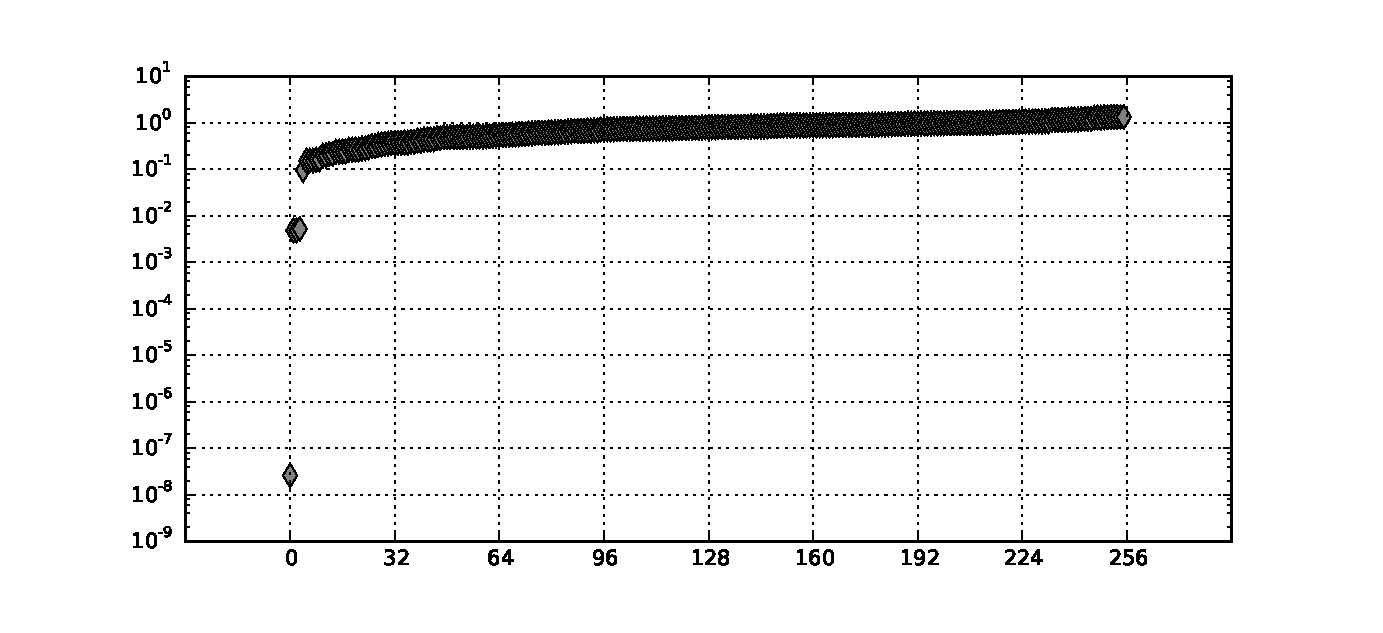
\includegraphics[width=\textwidth]{images/oscvalues.eps}
  \caption{The sorted magnitudes of the oscillatory parts of $\theta\big(
    \boldsymbol{h}_j - \tfrac{1}{2}\Abel_0^{\DivC}, \Omega \big)$ for each of
    the 256 half-lattice vectors $\boldsymbol{h}_j$. Note that the half-lattice
    vector resulting in the correct RCV produces a theta value approximately
    five orders of magnitude closer to zero than the others.}
  \label{fig:oscvalues}
\end{figure}

Even with the default numerical integration and Riemann theta accuracy of
$10^{-8}$ the choice of half-lattice vector producing the above RCV results in a
Riemann theta value that is several orders of magnitude closer to zero than with
the incorrect choices of half-lattice vector, as shown in Figure
\ref{fig:oscvalues}.

Let $\DivD$ be the divisor consisting of the three places lying above $x=2$ each
of multiplicity one. $\DivD$ is an effictive divisor of degree $g-1 = 3$.
Therefore, $\RCV(P_0) + \Abel(P_0,\DivD)$ is also a member of the theta divisor.
\begin{lstlisting}
sage: D = sum(places_above_two)
sage: W = J(AbelMap(D) + K(P0))
sage: v = RiemannTheta.oscillatory_part(W, Omega)
sage: abs(v)
1.09506634962e-10
\end{lstlisting}
\end{example}



%%% Local Variables:
%%% mode: latex
%%% TeX-master: "../thesis"
%%% End:
